\documentclass[12pt]{article}
\usepackage[utf8]{inputenc}
\usepackage[english]{babel}
\usepackage{cite}
\usepackage[]{amsthm} %lets us use \begin{proof}
\usepackage[]{amssymb} %gives us the character \varnothing
\usepackage[ruled,vlined]{algorithm2e}
\usepackage{listings}
\usepackage[utf8]{inputenc}
\usepackage{hyperref} 
\usepackage{amsmath}
\usepackage{csvsimple}
\usepackage{graphicx}
% One inch margins
\PassOptionsToPackage{margin=0.75in}{geometry}
\title{Modern Optimization Final Exam}
\author{Guanhua Huang}
\date\today

\begin{document}
\maketitle %This command prints the title based on information entered above
All the source code is stored at \url{https://github.com/victorhuangkk/york_optimization_final}

\begin{section}{Problem 12}
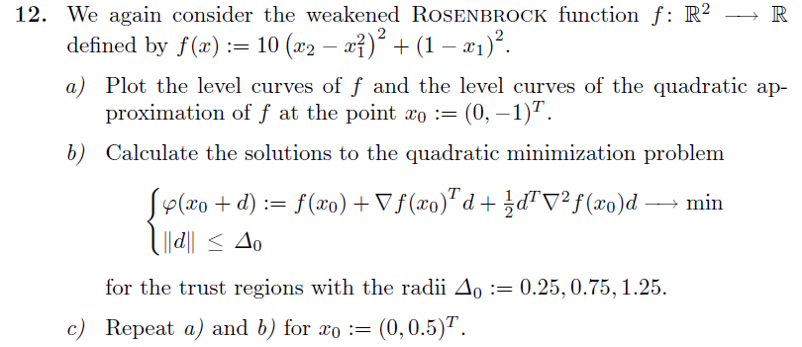
\includegraphics[width=10cm]{problem12.png}

\subsection{Part a}
\subsection{Part b}
\subsection{Part c}
\end{section}

\begin{section}{Problem 13}

   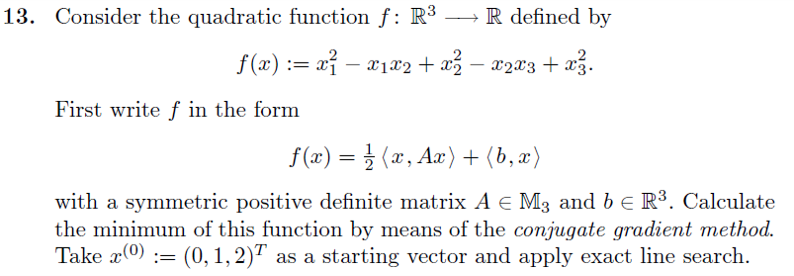
\includegraphics[width=10cm]{problem13.png}

    First, let's calculate A and b from the given formula:
    \[f(x) = \frac{1}{2}(x_1, x_2, x_3) \begin{pmatrix}
    a_1 & a_2 & a_3\\
    a_2 & a_4 & a_5 \\
    a_3 & a_5 & a_6 \end{pmatrix}
    \begin{pmatrix}
    x_1\\ 
    x_2 \\ x_3
    \end{pmatrix} + (b_1, b_2, b_3) \begin{pmatrix}
    x_1\\ x_2\\x_3  \end{pmatrix}\]
    
    Since there is no first order term in the final section, so, $b = (0, 0, 0)^T$
    \[\frac{1}{2}(a_1x_1+a_2x_2+a_3x_3, a_2x_1+a_4x_2+a_5x_3, a_3x_1+a_5x_2+a_6x_3)  \begin{pmatrix}
    x_1\\ 
    x_2 \\ x_3
    \end{pmatrix}\]
    
    \[=\frac{1}{2}x_1(a_1x_1+a_2x_2+a_3x_3) + 
    \frac{1}{2}x_2(a_2x_1+a_4x_2+a_5x_3) + 
    \frac{1}{2}x_3(a_3x_1+a_5x_2+a_6x_3)\]
    
    \[=\frac{1}{2}a_1x_1^2 + \frac{1}{2}a_4x_2^2 + \frac{1}{2}a_6x_3^2 + a_2x_1x_2 + a_3x_1x_3 + a_5x_2x_3\]
    \[=x_1^2 -x_1x_2 + x_2^2 -x_2x_3 + x_3^2\]
    
    For this reason, we know 
    $$A = \begin{pmatrix}
    	2 & -1 & 0\\
    	-1 & 2 & -1 \\
    	 0  & -1 & 2 \end{pmatrix}, \;\;\; b = \begin{pmatrix}
    	  0\\
    	  0 \\
    	  0 \end{pmatrix}$$
    
    The implementation is done in python and I pasted the code here for reference purposes. 
    \lstinputlisting[language=python]{cg_algo.py}
    
    And the execution results is 

   	\begin{tabular}{llll}
   		\hline
   		Iteration & $x_0$ & $x_1$& $x_2$ \\
   		\hline\hline
   		0 & 0     & 1     & 2     \\
   		1 & 0.5   & 1     & 0.5   \\
   		2 & 0.556 & 0.444 & 0.333 \\
   		3 & 0     & 0     & 0    
   	\end{tabular}

\end{section}

\begin{section}{Problem 15}
	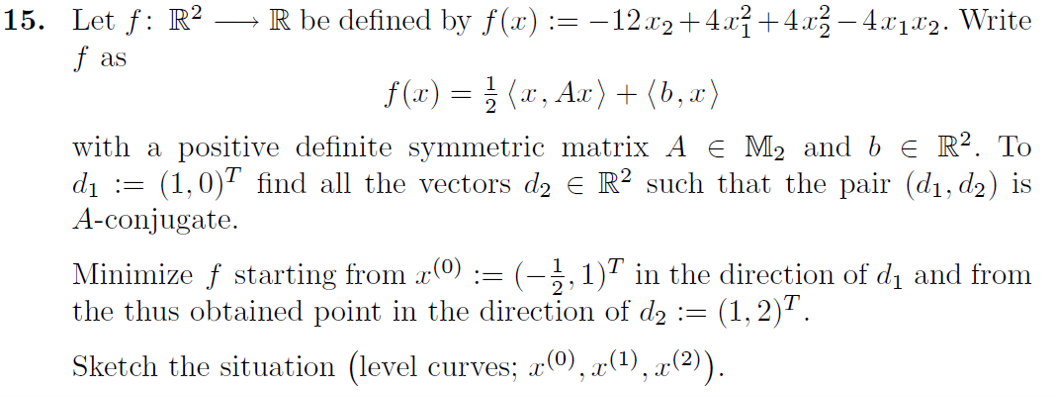
\includegraphics[width=12cm]{problem15.png}

	\subsection{Part 1}
	First, let's write the matrix format of the function,

	$$\frac{1}{2} (x_1, x_2) \begin{pmatrix}
	a_1 & a_2\\
	a_2 & a_3 \end{pmatrix}
	\begin{pmatrix}
	x_1\\ 
	x_2
	\end{pmatrix} + (b_1, b_2) \begin{pmatrix}
	x_1\\
	x_2
	\end{pmatrix}$$
	\[= \frac{1}{2}(a_1x_1 + a_2x_2, a_2x_1+a_3x_2) \begin{pmatrix}
	x_1\\
	x_2
	\end{pmatrix} + x_1b_1 + x_2b_2\]
	\[= \frac{1}{2}(a_1x_1 + a_2x_2)x_1 + \frac{1}{2}(a_2x_1 + a_3x_2)x_2 + x_1b_1 + x_2b_2\]
	\[= \frac{1}{2}a_1x_1^2 + a_2x_1x_2 + \frac{1}{2}a_3x_2^2 + b_1x_1 + b_2x_2\]
	\[=-12x_2 + 4x_1^2 + 4x_2^2-4x_1x_2\]	

	By comparing parameters, we got the following, 
	\[b_2 = -12, b_1 = 0, a_2 = -4, a_1 =a_3 = 8\]
	\[A = \begin{pmatrix}
	8 & -4\\
	-4 & 8
	\end{pmatrix}, b = \begin{pmatrix}
	0\\
	-12
	\end{pmatrix}\]
	
	Based on A-conjugate definition (on page 120), $\langle d_1, Ad_2 \rangle = 0, \;\; d_1 = (1,0)^T$, then, let's write out the problem as the following: 
	
	$$(1,0) \begin{pmatrix}
	8 & -4\\
    -4 & 8 \end{pmatrix} \begin{pmatrix}
	\delta_1\\
     \delta_2 \end{pmatrix} = (8, -4) \begin{pmatrix}
     \delta_1\\
     \delta_2 \end{pmatrix} = 8\delta_1 - 4\delta_2 = 0$$
    So, as long as $2\delta_1 = \delta_2$, the condition $\langle d_1, Ad_2 \rangle = 0$ is satisfied
    $$d_2 = \begin{pmatrix}
    \gamma\\
    2\gamma \end{pmatrix}, \;\; \forall \gamma \in \mathbb{R}$$	
	\subsection{Part 2}
	
	Let's calculate the gradient of the function,
	\[f(x) = -12x_2 + 4x_1^2 + 4x_2^2-4x_1x_2, \;\; \nabla f(x) = \begin{pmatrix}
	8x_1 - 4x_2\\
	-12 + 8x_2 - 4x_1 \end{pmatrix} = g(x)\]
	
	Then, we can evaluate $g_0 = \begin{pmatrix}
	-\frac{1}{2} \times 8 - 4 \times 1\\
	-12 + 8 + 2
	\end{pmatrix} = \begin{pmatrix}
	-8\\
	-2
	\end{pmatrix}$ by given $x_0 = \begin{pmatrix}
	-\frac{1}{2}\\
	1
	\end{pmatrix}$
	
	In this problem, $d_1$ is given so we don't have to calculate it by $g_0$. So, the next stuff we need is the $\lambda_0 = -\frac{ \langle g_0, d_0 \rangle}{\langle Ad_0, d_0\rangle}$. I would calculate the numerator and enumerator separately.
	
	\[-\langle g_0, d_0 \rangle = -(-8, -2) \begin{pmatrix}
	1\\
	0
	\end{pmatrix} = 8\] 
	\[\langle Ad_0, d_0 \rangle  = (1,0) \begin{pmatrix}
	8 & -4\\
	-4 & 8
	\end{pmatrix} \begin{pmatrix}
	1\\
	0
	\end{pmatrix} = (8, -4) \begin{pmatrix}
	1\\
	0
	\end{pmatrix} = 8\]
	
	For this reason, $\lambda_0 = \frac{8}{8}=1$, and $x^{(1)}$ is, 
	\[x^{(1)} = \begin{pmatrix}
	-1/2\\
	1
	\end{pmatrix} + 1 \begin{pmatrix}
	1\\
	0
	\end{pmatrix} = \begin{pmatrix}
	\frac{1}{2}\\
	1
	\end{pmatrix} \]
	
	In the next iteration, we calculate $x^{(2)}$. To accomplish that, we calculate $g_1 = \begin{pmatrix}
	\frac{1}{2} \times 8 - 4 \times 1\\
	-12 + 8 - 4 \times \frac{1}{2}
	\end{pmatrix} = \begin{pmatrix}
	0\\
	-6
	\end{pmatrix}$
	
	and by given in the problem, we know $d_1 = \begin{pmatrix}
	1\\
	2
	\end{pmatrix}$, I follow the same routine to calculate the $\lambda_1$
	\[-\langle g_1, d_1 \rangle = -(0, -6) \begin{pmatrix}
	1\\
	2
	\end{pmatrix} = 12\] 
	
	\[\langle Ad_0, d_0 \rangle  = (1,2) \begin{pmatrix}
	8 & -4\\
	-4 & 8
	\end{pmatrix} \begin{pmatrix}
	1\\
	2
	\end{pmatrix} = (0, 12) \begin{pmatrix}
	1\\
	2
	\end{pmatrix} = 24\]
	
	For this reason, $\lambda_1 = \frac{1}{2}$ and we can evaluate $x^{(2)}$ as
	\[x^{(2)} = \begin{pmatrix}
	1/2\\
	1
	\end{pmatrix} + \frac{1}{2} \begin{pmatrix}
	1\\
	2
	\end{pmatrix} = \begin{pmatrix}
	1\\
	2
	\end{pmatrix} \]
	 
	\subsection{Part 3}
	The visualization has been done in python via matplotlib. Please refer to the source code to see details. Here is the plot. 
		\begin{figure}[htp]
		\centering
		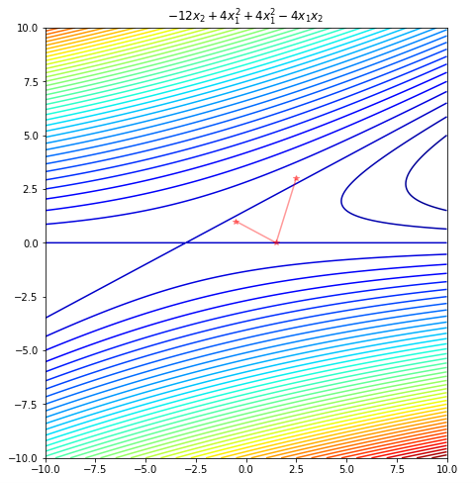
\includegraphics[width=12cm]{problem15_plt1.png}
	\end{figure}

\end{section}

\begin{section}{Problem 18}
	\subsection{Part a}
	First, I tested all available methods in scipy with tolerance $10^{-6}$. All results are summarized below. Since the Gradient (Jacobian) is not provided in this case, some methods through out error messages. It will be discussed later in the problem. 
	
	
		\begin{tabular}{lllll}
			\hline
			Method & NIterations & $x_1$ & $x_2$& Final Function Value \\
			\hline\hline
			Nelder-Mead  & 58  & 2.541  & 0.26     & 2.247    \\
			Powell       & 8   & 2.541  & 0.26     & 2.247    \\
			CG           & 0   & 3      & 0.5      & 10805.97 \\
			BFGS         & 32  & 2.541  & 0.26     & 2.247    \\
			TNC          & 10  & 2.54   & 0.26     & 2.247    \\
			L-BFGS-B     & 16  & 2.541  & 0.26     & 2.247    \\
			TNC          & 10  & 2.54   & 0.26     & 2.247    \\
			trust-constr & 986 & 2.541  & 0.26     & 2.247    \\
			SLSQP        & 2   & -5.104 & -189.594 & 291     
		\end{tabular}
	
    
    From the table, we know that some algorithms did a good jon but some doesn't. Then, let's give the gradient to the method and do another round. 
    
    	\begin{tabular}{lllll}
    		\hline
    		Method & NIterations & $x_1$ & $x_2$& Final Function Value \\
    		\hline\hline
    		Nelder-Mead  & 58 & 2.541    & 0.26    & 2.247    \\
    		Powell       & 8  & 2.541    & 0.26    & 2.247    \\
    		CG           & 4  & 1.011    & 0.382   & 13.499   \\
    		BFGS         & 2  & 2.698    & -18.447 & 291      \\
    		Newton-CG    & 24 & 1.055    & 0.378   & 12.91    \\
    		L-BFGS-B     & 8  & 1.098    & 0.373   & 12.142   \\
    		TNC          & 1  & -1.136   & 0.475   & 2908.226 \\
    		trust-constr & 24 & 1.029    & 0.381   & 13.289  \\
    		SLSQP        & 2  & -187.094 & -7.604  & 291.284  
    	\end{tabular}

	CG, Newton-CG, SLSQP, dogleg, trust-ncg, trust-krylov, and trust-exact require the gradient input. 
	\subsection{Part b}
	The least square result is summarized here 
	
	\subsection{Part c}
	The visualization is in the previous two parts already. Please refer there to see summaries. And in terms of source code, please refer to github or the other files. 
\end{section}




\end{document}